\documentclass[11pt]{article}
\usepackage{latexsym}
\usepackage{amsmath}
\usepackage{amssymb}
\usepackage{amsthm}
\usepackage{epsfig}
\usepackage{bm}
\usepackage{scrextend}
\usepackage[tight]{subfigure}
\usepackage{physics}

\usepackage{amsmath}
% \usepackage{algorithmicx}
\usepackage{algorithm}
\usepackage{algpseudocode}

\DeclareMathOperator*{\minimize}{min}
\DeclareMathOperator*{\maximize}{max}
\DeclareMathOperator{\sign}{sign}

 %on linux you may need to run sudo apt-get install texlive-full to install algorithm.sys

\usepackage{verbatim}

\newcommand{\handout}[5]{
  \noindent
  \begin{center}
  \framebox{
    \vbox{
      \hbox to 5.78in { {#1} \hfill #2 }
      \vspace{4mm}
      \hbox to 5.78in { {\Large \hfill #5  \hfill} }
      \vspace{2mm}
      \hbox to 5.78in { {\em #3 \hfill #4} }
    }
  }
  \end{center}
  \vspace*{4mm}
}

\newcommand{\lecture}[5]{\handout{#1}{#2}{#3}{#4}{#5}}
\newcommand{\collision}[0]{\mathrm{collision}}
\newcommand{\nocollision}[0]{\overline{\collision}}
\newcommand{\argmax}[1]{\underset{#1}{\operatorname{arg}\,\operatorname{max}}\;}
\newcommand{\argmin}[1]{\underset{#1}{\operatorname{arg}\,\operatorname{min}}\;}

\newcommand*{\QED}{\hfill\ensuremath{\square}}

\newtheorem{theorem}{Theorem}
\newtheorem{corollary}[theorem]{Corollary}
\newtheorem{lemma}[theorem]{Lemma}
\newtheorem{observation}[theorem]{Observation}
\newtheorem{proposition}[theorem]{Proposition}
\newtheorem{definition}[theorem]{Definition}
\newtheorem{claim}[theorem]{Claim}
\newtheorem{fact}[theorem]{Fact}
\newtheorem{assumption}[theorem]{Assumption}
\newtheorem{note}[theorem]{Note}


% 1-inch margins, from fullpage.sty by H.Partl, Version 2, Dec. 15, 1988.
\topmargin 0pt
\advance \topmargin by -\headheight
\advance \topmargin by -\headsep
\textheight 8.9in
\oddsidemargin 0pt
\evensidemargin \oddsidemargin
\marginparwidth 0.5in
\textwidth 6.5in

\parindent 0in
\parskip 1.5ex
%\renewcommand{\baselinestretch}{1.25}

\begin{document}

\lecture{Statistical Techniques in Robotics (16-831, S21)}{Lecture \#08
  (Monday, March 1)}{Lecturer: Kris Kitani}{Scribes: Haowen Shi, Fan Jia}{Online Convex Optimization (OMD, Duality, Regret)}

\section{Review}
%This section serves as a review of the previous lecture and any other context required to frame the content of the current lecture. 

%You may format the scribes in any way you like, aside from changing font style, size and page format. Please use subsections and paragraphs to increase the readability of your notes.
Previously we studied Follow The Leader (FTL) and Follow The Regularized Leader (FTRL) algorithms in the Online Convex Optimization (OCO) \cite{shalev2011online} category.
\subsection{Follow The Leader with Quadratic Loss}
\begin{algorithm}
  \caption{FTL with Quadratic Loss}\label{euclid}
  \begin{algorithmic}[1]
    \Function{Follow the leader (Quadratic Loss)}{} %\Comment{The g.c.d. of a and b}
    \State $f^{(0)} \leftarrow 0$
        \For{$t=1, 2,\,\cdots,\;T$}
            \State $\bm{w}^{(t)}$ = $\argmin{\bm{w} \in S} \Sigma^{t-1}_{i=1} f^{(i)} (\bm{w})$ 
            \State \textsc{Receive} ($f^{(t)} = \frac{1}{2}||\bm{w} - \bm{z}^{(t)}||_2^2$) \Comment{Receive loss function}
        \EndFor
    \EndFunction
  \end{algorithmic}
\end{algorithm}
We proved the regret bound is:
\begin{equation*}
    \text{Regret} \leq 4L^2 \left( \log(T) + 1 \right)
\end{equation*}
This is no-regret since the average regret grows sub-linearly in T. However, this only holds for quadratic loss functions, not for all convex functions.

\subsection{Follow The Leader with Linear Loss}
\begin{algorithm}
  \caption{Follow the leader algorithm with linear loss}\label{euclid}
  \begin{algorithmic}[1]
    \Function{Follow the leader (Linear Loss)}{} %\Comment{The g.c.d. of a and b}
        \For{$t=1, 2,\,\cdots,\;T$}
            \State $\bm{w}^{(t)}$ = $\argmin{\bm{w} \in S} \left(\Sigma^{t-1}_{i=1} \bm{z}^{(i)}\right) \cdot \bm{w}$ 
            \State \textsc{Receive} ($f^{(t)}(\bm{w}) = \bm{z}^{(t)} \cdot \bm{w}$) \Comment{Receive loss function}
        \EndFor
    \EndFunction
  \end{algorithmic}
\end{algorithm}

We observed that the regret of FTL with linear loss relative to an expert $u$ that chooses $w=0$ is:
\begin{equation*}
    \text{Regret}(u) = T-1-0 = T-1 = O(T)
\end{equation*}
The regret grows linearly because the $\bm{w}$ value flip-flops back and forth and make the algorithm unstable. To resolve this issue, we introduced regularization.

\subsection{Follow The Regularized Leader}
\begin{algorithm}
  \caption{Follow The Regularized Leader}\label{euclid}
  \begin{algorithmic}[1]
    \Function{FTRL(Convex Set $\mathcal{S}$)}{} %\Comment{The g.c.d. of a and b}
    \For{$t=1, 2,\,\cdots,\;T$}
        \State $\bm{w}^{(t)}$ = $\argmin{\bm{w} \in S} \Sigma^{t-1}_{i=1} f^{(i)} (\bm{w}) + \psi(\bm{w})$
        \Comment{Added $\psi(\bm{w})$ to the prediction rule}
        \State \textsc{Receive} ($f^{(t)} : \mathcal{S} \rightarrow \mathbb{R}$)
    \EndFor
    \EndFunction
  \end{algorithmic}
\end{algorithm}
We proved the regret bound for FTRL is:
\begin{align*}
    R(\bm{u}) &\triangleq \sum_{t=1}^{T} \left[ f^{(t)}(\bm{w}^{(t)}) - f^{(t)}(\bm{u}) \right]\\
    & \leq \left[ \psi(\bm{u}) - \psi(\bm{w}^{(1)}) \right] +  \sum_{t=1}^{T} \left[ f^{(t)}(\bm{w}^{(t)}) - f^{(t)}(\bm{w}^{(t+1)}) \right]
\end{align*}

\begin{algorithm}[h]
  \caption{FTRL with Linear Loss And Quadratic Regulation}\label{euclid}
  \begin{algorithmic}[1]
    \Function{FTRL(Convex Set $\mathcal{S}$)}{} %\Comment{The g.c.d. of a and b}
    \For{$t=1, 2,\,\cdots,\;T$}
        \State $\bm{w}^{(t)}$ = $\argmin{\bm{w} \in S} \Sigma^{t-1}_{i=1} \left( \frac{1}{2\eta} ||\bm{w}||^2_2 + \bm{w} \cdot \sum_{i=1}^{t-1} z^{(i)} \right)$
        \Comment{Prediction rule}
        \State \textsc{Receive} ($f^{(t)} : \bm{w} \cdot z^{(t)}$)
    \EndFor
    \EndFunction
  \end{algorithmic}
\end{algorithm}
We proved the regret bound for FTRL with a Euclidean regularizer and linear loss function is:
\begin{equation*}
    \label{eqn:ftrl_regret_bound_euclidean}
    R^{(T)}(\bm{u}) \leq BL\sqrt{2T}
\end{equation*}
Where $L = \max_\mathcal{Z} || \mathcal{Z} ||_2$ and $B = \max_{\bm{u} \in \mathcal{S}} || \bm{u} ||_2$.

\textit{Online Mirror Descent} (OMD) can be considered as a special case of FTRL with a linear loss and a convex regularizer. In this lecture, we will focus on OMD.

\section{Online Mirror Descent}

\textit{Online Mirror Descent} (OMD) \cite{lan2012validation} can be considered as a special case of FTRL. Fig. \ref{fig:ftl_ftrl_omd} shows the relationship between FTL, FTRL and OMD. FTRL adds a regularizer by forcing the zero-step loss to be a non-zero regularization function $\psi(\bm{w})$. In particular, if a FTRL problem has a convex regularization $\psi(\bm{w})$ and a linear loss function, it is called OMD.

\begin{figure}[h]
    \centering
    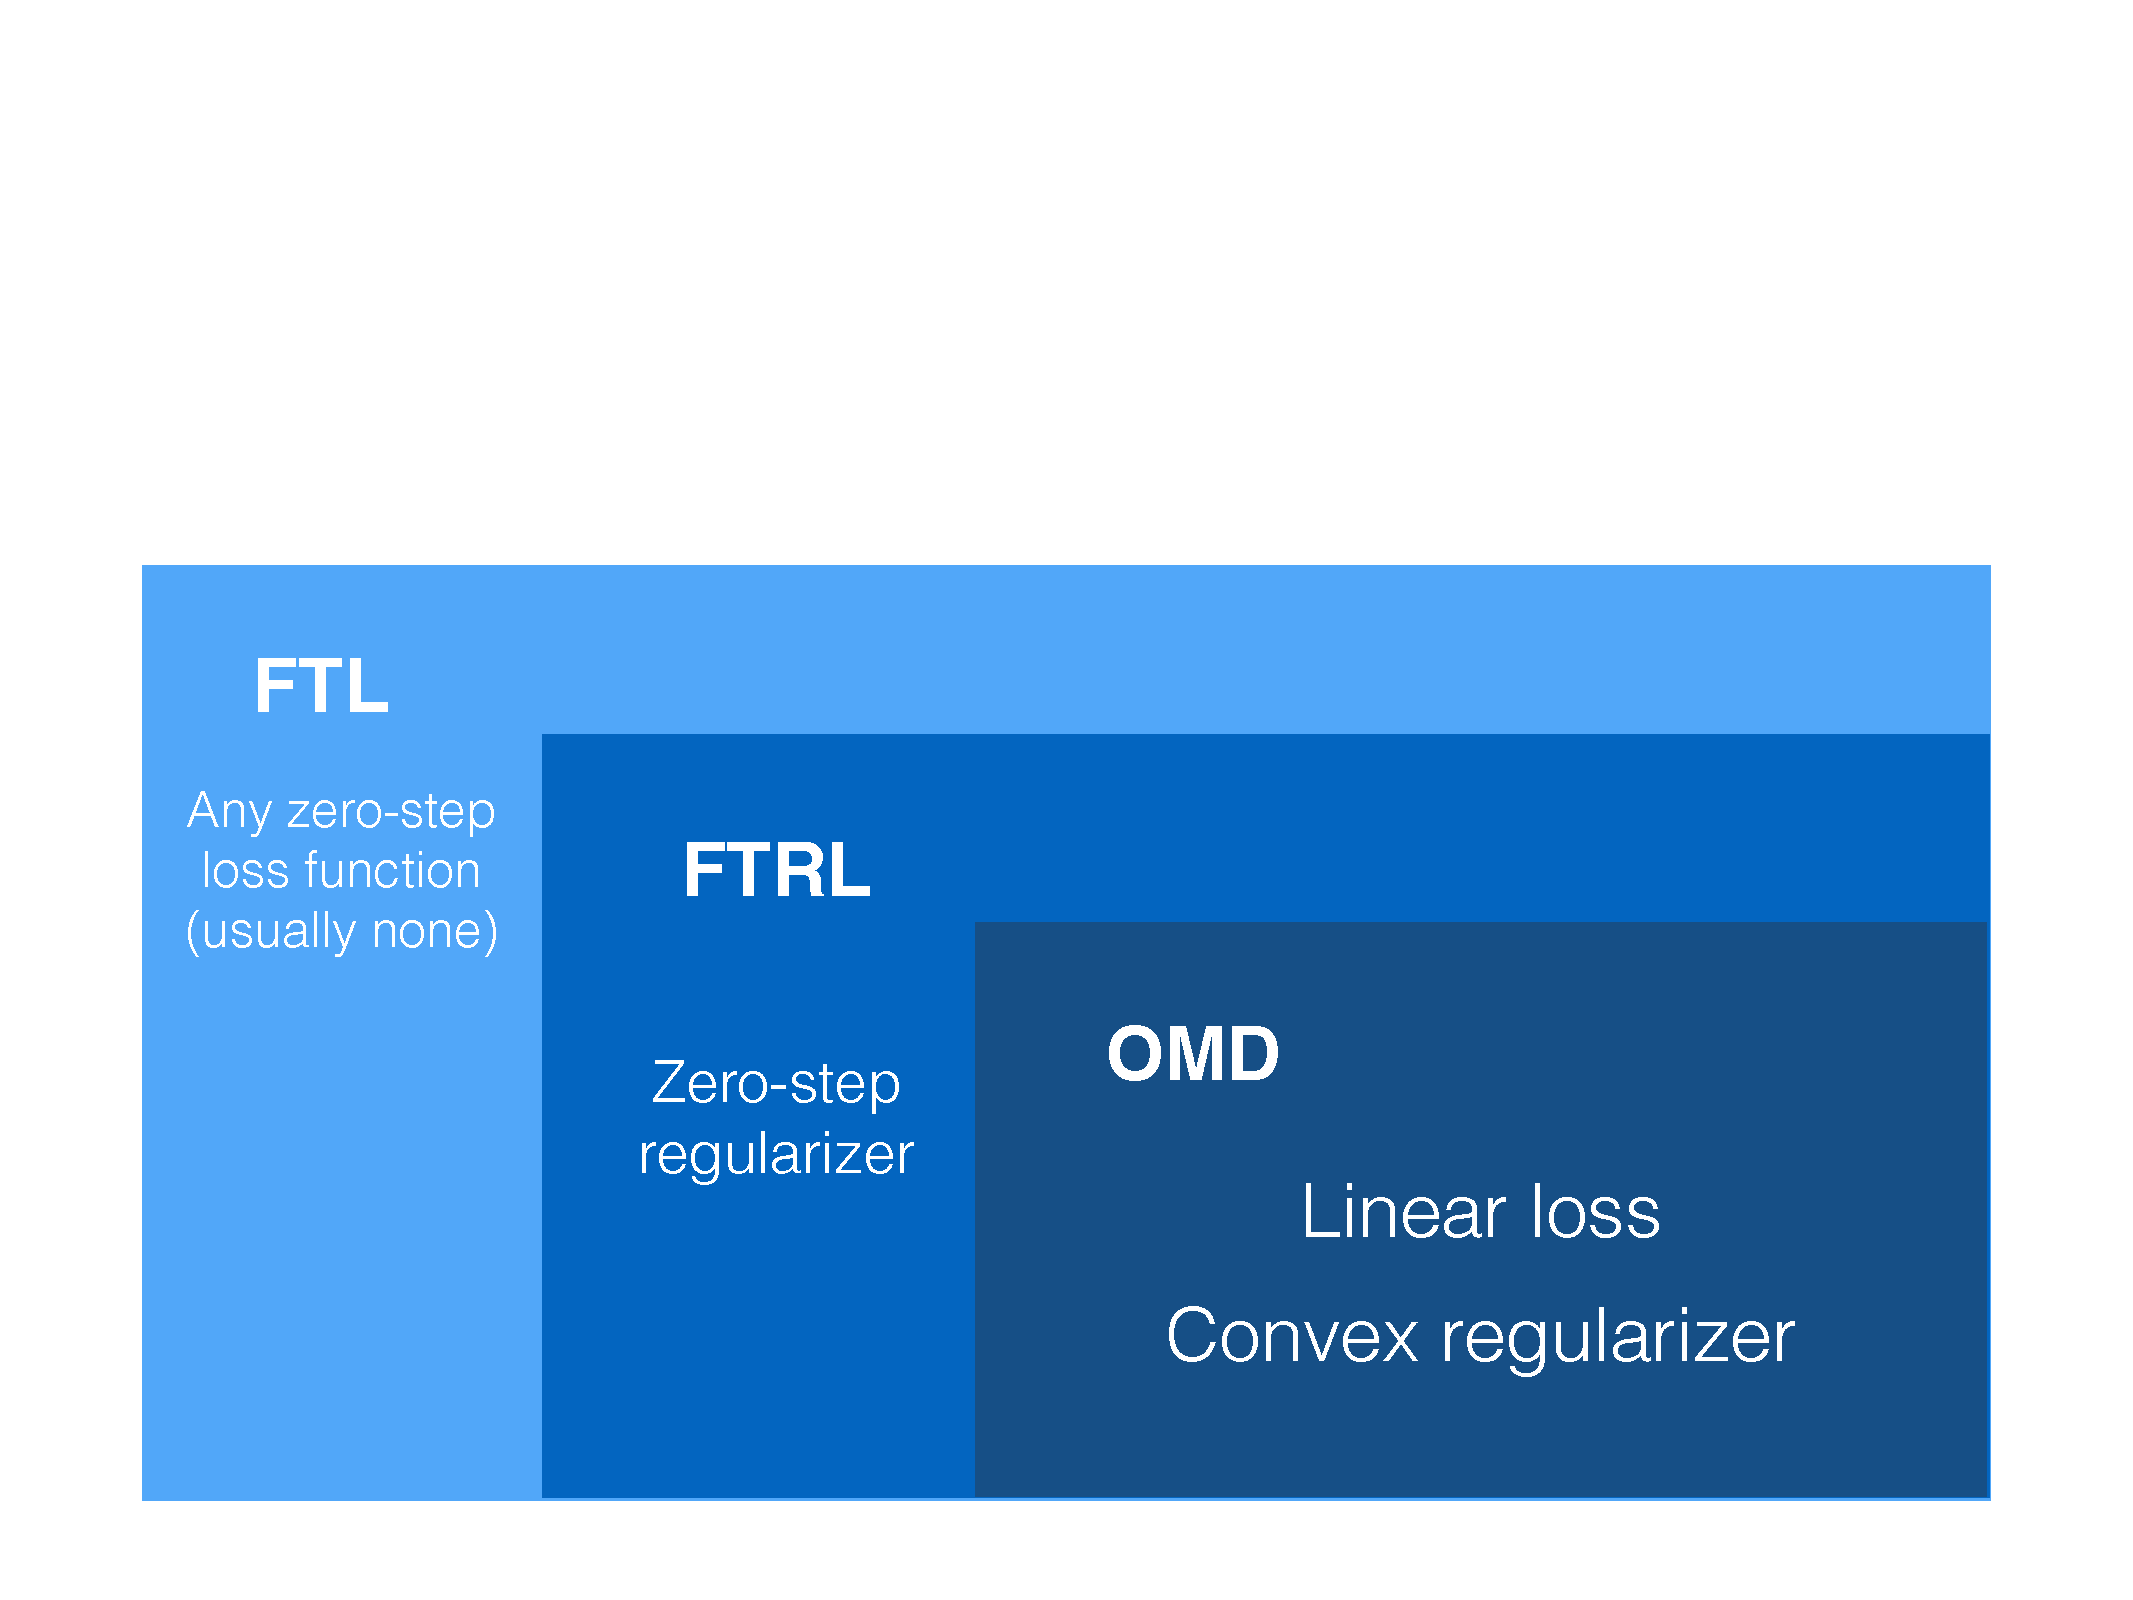
\includegraphics[width=0.5\textwidth]{figures/ftl_ftrl_omd.pdf}
    \caption{OMD can be seen as FTRL with convex regularization and linear loss}
    \label{fig:ftl_ftrl_omd}
\end{figure}

With a linear loss, we can write the loss function as a dot product (linear combination) of the loss function parameter $\bm{z}$ and primal space parameter $\bm{w}$, as shown in Algorithm \ref{algo:ftrl_lin_loss}.

\begin{algorithm}
  \caption{Follow The Regularized Leader - Linear Loss}
  \label{algo:ftrl_lin_loss}
  \begin{algorithmic}[1]
    \Function{FTRL-LinLoss(Convex Set $\mathcal{S}$)}{}
    \For{$t=1, 2,\,\cdots,\;T$}
        \State $\bm{w}^{(t)}$ = $\argmin{\bm{w} \in S} \Sigma^{t-1}_{i=1} \langle \bm{w}, \bm{z}^{(i)} \rangle + \psi(\bm{w})$
        \Comment{Added $\psi(\bm{w})$ to the prediction rule}
        \State \textsc{Receive} ($f^{(t)} : \mathcal{S} \rightarrow \mathbb{R}$)
    \EndFor
    \EndFunction
  \end{algorithmic}
\end{algorithm}

We generalize \texttt{FTRL-LinLoss} to derive OMD. First, we define some notations:
\begin{align}
    \intertext{Denote sum of $\bm{z}$:}
    \bm{z}^{(1:t)} &= \sum_{i=1}^t \bm{z}^{(i)}
    \intertext{Define parameter of the dual space $\bm{\theta}$:}
    \bm{\theta}^{(t+1)} &\triangleq - \bm{z}^{(1:t)}
    \label{eqn:dual_space}
    \intertext{So we have the following update in each iteration for $\bm{\theta}$:}
    \bm{\theta}^{(t+1)} &= \bm{\theta}^{(t)} - \bm{z}^{(t)}
\end{align}
Then, because the loss function $f^{(i)}$ is linear, we can generalize the FTRL prediction step as follows:
\begin{align*}
    \bm{w}^{(t+1)} &= \argmin{\bm{w}} \sum_{i=1}^t f^{(i)}(\bm{w})
    + \psi(\bm{w})
    & \text{FTRL prediction step}\\
    &= \argmin{\bm{w}} \langle \bm{w}, \bm{z}^{(1:t)} \rangle
    + \psi(\bm{w})
    & \text{Linear loss function}\\
    &= \argmax{\bm{w}} \langle \bm{w}, -\bm{z}^{(1:t)} \rangle
    - \psi(\bm{w})
    & \text{Convert to maximization}\\
    &= \argmax{\bm{w}} \langle \bm{w}, \bm{\theta}^{(t+1)} \rangle
    - \psi(\bm{w})
    & \text{Substitute (\ref{eqn:dual_space})}\\
    &= g(\bm{\theta}^{(t+1)})
    & \text{$g$: mirror/linking function}
\end{align*}

The function $g : \bm{\theta} \rightarrow \bm{w}$ is called the mirror/linking function because it takes parameters from the dual space ($\bm{\theta}$) and maps to the primal space ($\bm{w}$). This function is where the ``mirror'' name in the OMD came from. With the definitions introduced above, we can change some notations (without changing the algorithm itself) and re-write Algorithm \ref{algo:ftrl_lin_loss} as:

\begin{algorithm}
  \caption{Online Mirror Descent}
  \label{algo:omd}
  \begin{algorithmic}[1]
    \Function{OMD(Convex Set $\mathcal{S}$, $g:\mathbb{R}^D \rightarrow \mathcal{S}$)}{}
    \For{$t=1, 2,\,\cdots,\;T$}
        \State \textsc{Receive} ($f^{(t)}:\mathcal{S}\rightarrow \mathbb{R}$)
        \State $\bm{\theta}^{(t+1)} = \bm{\theta}^{(t)} - \eta \bm{z}^{(t)}$, $\bm{z} \in \partial f^{(t)}(\bm{w}^{(t)})$
        \Comment Dual parameter update
        \State $\bm{w}^{(t+1)} = g(\bm{\theta}^{(t+1)})$
        \Comment Primal parameter update (or mirror projection)
    \EndFor
    \EndFunction
  \end{algorithmic}
\end{algorithm}

The regret bound of OMD (discussed in section \ref{sec:omd_regret}) shares the same structure with FTRL because at the core they are the same algorithm. With OMD we are doing optimization in the dual space and map back to the primal space to get the updated parameter that we are optimizing (as illustrated in Fig. \ref{fig:dual_primal}). The benefit of introducing dual space is primarily for theoretical purposes. By looking at the optimization in a different space, we can better understand optimization in the primal space and make more informed changes and improvements.

\begin{figure}[h]
    \centering
    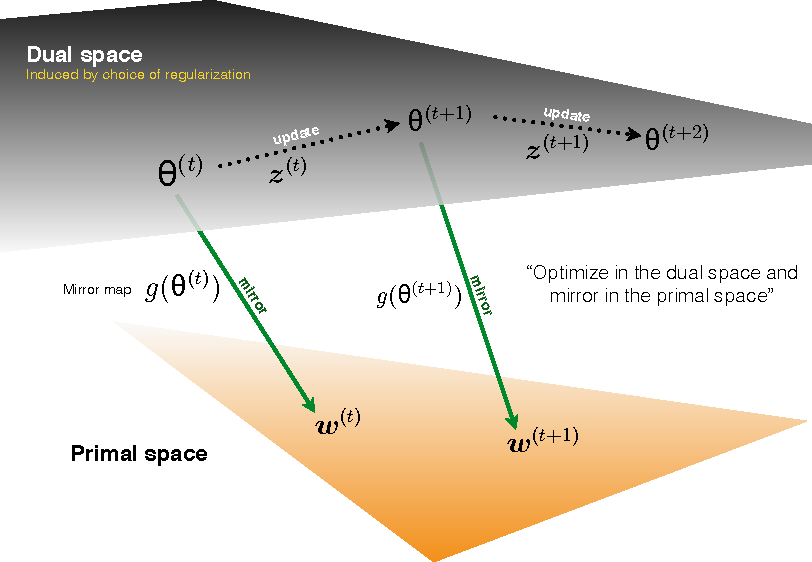
\includegraphics[width=0.8\textwidth]{figures/dual_primal.pdf}
    \caption{Illustration of online mirror descent in the dual space}
    \label{fig:dual_primal}
\end{figure}

A different regularization function $\psi$ leads to a different mirror function $g$. The regularization should be chosen such that the mirroring can take better advantage of the ``geometry'' of the problem.

\section{Duality}
In this section we introduce mathematical tools that help us analyze OMD.

\subsection{Convex Conjugate}
A \textit{convex conjugate} function is also called a Fenchel dual / a Fenchel conjugate / a Fenchel transform \cite{wiki:convex_conjugate}. Here we focus on conjugate functions assuming a smooth convex function. The generalized version of this process for non-smooth and non-convex functions is called a Legendre transformation. The definition for a convex conjugate function is:
\begin{equation}
    \label{eqn:convex_conjugate}
    \psi^* (\theta) = \max_w (\langle \theta, w \rangle - \psi(w))
\end{equation}

For better understanding, the geometric interpretation of convex conjugate is included in the appendix section \ref{sec:convex_conjugate_geometric}.
Given (\ref{eqn:convex_conjugate}), we can derive some useful properties used to analyze the regret of OMD:
\begin{align}
    \intertext{Derivative of convex conjugate:}
    \nabla_{\bm{\theta}} \psi^* (\bm{\theta})
    &= \frac{\partial \psi^*(\bm{\theta})}{\partial \bm{\theta}}
    = \bm{w}^* = \argmax{w}
    (\langle \bm{\theta}, \bm{w} \rangle - \psi(\bm{w}))
    \label{eqn:conjugate_deriv_2}\\
    \nabla_{\bm{w}} \psi(\bm{w})
    &= \eval{\frac{\partial \psi(\bm{w})}{\partial \bm{w}}}_{\bm{w}=\bm{w}^*} = \bm{\theta}
    \intertext{Fenchel-Young inequality:}
    \psi^*(\bm{\theta}) &\geq (\langle \bm{w}, \bm{\theta} \rangle - \psi(\bm{w}))
    \label{eqn:conjugate_fenchel_young}
\end{align}
The proof for (\ref{eqn:conjugate_deriv_2}) is in section \ref{sec:proof_prop_conjugate}. The proof for (\ref{eqn:conjugate_fenchel_young}) is trivial because any $w$ other than the optimal $w^*$ will produce less distance $\psi$ than maximum $\psi^*$ according to the maximizer definition (\ref{eqn:convex_conjugate}).

\subsection{Bregman Divergence}
Bregman divergence is the approximation error of the first order approximation of $\psi(\bm{w})$ at $\bm{u}$.
\begin{equation*}
    D_{\psi}(\bm{w}||\bm{u}) = \psi(\bm{w}) - \psi(\bm{u}) - \nabla\psi(\bm{u})^\top(\bm{w}-\bm{u})
\end{equation*}

The geometric interpretation of Bregman divergence is included in the appendix section \ref{sec:bregman_divergence_geometric}.


\section{OMD Regret Analysis}
\label{sec:omd_regret}
We analysis the regret bound of the OMD algorithm in this section. The regret is:
\begin{equation*}
    R(\bm{u}) = \sum_{t=1}^{T} \bm{w}^{(t)} \cdot \bm{z}^{(t)} - \bm{u} \cdot \bm{z}^{(t)}
\end{equation*}
where $\bm{z}$ is the derivative of the loss function. The following regret bound holds for any OMD algorithm:

\begin{equation*}
    R(\bm{u}) \leq \psi(\bm{u}) - \psi(\bm{w}^{(1)}) + \sum_{t=1}^{T} D_{\psi^*}(-\bm{z}^{(1:t)}||-\bm{z}^{(1:t-1)})
\end{equation*}
The regret is upper bounded by the sum of the difference in the regularization function plus the sum of all Bregman divergence under the convex conjugate of the regularization function. The proof is as follows:

\begin{proof}
The loss of an arbitrary vector $\bm{u}$:
\begin{equation*}
    \psi(\bm{u}) + \sum_{t=1}^{T} \bm{u} \cdot \bm{z}^{(t)} = \psi(\bm{u}) - \bm{u} \cdot \bm{\theta}^{T+1}
\end{equation*}
where $\bm{\theta}^{T+1}$ is the sum of gradients till to time step $T$.\\[3pt]
Recall Fenchel-Young Inequality:
\begin{equation*}
    \psi^* (\bm{\theta}) \geq (\langle \bm{w}, \bm{\theta} \rangle - \psi(\bm{w}))
\end{equation*}
Apply Fenchel-Young Inequality to the right hand side:
\begin{equation*}
    \psi(\bm{u}) - \bm{u} \cdot \bm{\theta}^{T+1} \geq -\psi^*(\bm{\theta}^{(T+1)})
\end{equation*}
Then we expand the right hand side with telescoping. A telescoping series is a series whose partial sums eventually only have a fixed number of terms after cancellation.\\[3pt]
Convert to telescoping series by adding and subtracting the complex conjugate at time step 1:
\begin{equation*}
    -\psi^*(\bm{\theta}^{(T+1)}) = -\psi^*(\bm{\theta}^{(T+1)})  -\psi^*(\bm{\theta}^{(1)}) + \psi^*(\bm{\theta}^{(1)})
\end{equation*}
Sum over shifted time steps:
\begin{equation*}
\begin{aligned}
    -\psi^*(\bm{\theta}^{(T+1)}) &= -\psi^*(\bm{\theta}^{(T+1)}) - \psi^*(\bm{\theta}^{(T)}) + \psi^*(\bm{\theta}^{(T)}) - \cdots -\psi^*(\bm{\theta}^{(1)}) + \psi^*(\bm{\theta}^{(1)})\\
    &= -\psi^*(\bm{\theta}^{(1)}) - \sum_{t=1}^T (\psi^*(\bm{\theta}^{(t+1)}) - \psi^*(\bm{\theta}^{(t)}))
    \end{aligned}
\end{equation*}
Plug in definition of Bregman divergence:
\begin{equation*}
    -\psi^*(\bm{\theta}^{(T+1)}) = -\psi^*(\bm{\theta}^{(1)}) - \sum_{t=1}^T \left( \nabla \psi^*(\bm{\theta}^{(t)}) \cdot (\bm{\theta}^{(t+1)} - \bm{\theta}^{(t)}) +  D_{\psi^*}(\bm{\theta}^{(t+1)}||\bm{\theta}^{(t)})\right)
\end{equation*}

The first term can be written as $\psi(\bm{w}^{(1)})$ since:
\begin{align*}
    \psi^*(\bm{\theta}^{(1)}) &= \psi^*(\bm{\bm{z}}^{(0)})
    & \text{from definition} \quad \bm{\theta}^{(t+1)} \triangleq - \bm{z}^{(1:t)} \\
    &= \psi^*(\bm{0})
    & \text{From definition of conjugate}\\
    &= \max_{\bm{w}} (\langle \bm{w}, \bm{0} \rangle
    - \psi(\bm{w}))
    & \text{Compute dot product}\\
    &= \max_{\bm{w}} (\bm{0} 
    - \psi(\bm{w}))
    & \text{Sign flip max-min conversion}\\
        &= -\min_{\bm{w}}
    \psi(\bm{w})
    & \text{Plug in minimizer of cumulative loss at time 1}\\
    &= -
    \psi(\bm{w}^{(1)})
    & \text{Minimizer is the primal iterate at step 1}\\
    & &\text{(`the one-step look ahead cheater')}
\end{align*}
Therefore, we have:
\begin{equation*}
    -\psi^*(\bm{\theta}^{(T+1)}) = \psi(\bm{w}^{(1)}) - \sum_{t=1}^T \left( \nabla \psi^*(\bm{\theta}^{(t)}) \cdot (\bm{\theta}^{(t+1)} - \bm{\theta}^{(t)}) +  D_{\psi^*}(\bm{\theta}^{(t+1)}||\bm{\theta}^{(t)})\right)
\end{equation*}
Plug in definition of dual parameter $\bm{\theta}^{(t+1)} \triangleq - \bm{z}^{(1:t)}$:
\begin{equation*}
    -\psi^*(\bm{\theta}^{(T+1)}) = \psi(\bm{w}^{(1)}) - \sum_{t=1}^T \left( \nabla \psi^*(-\bm{z}^{(1:t-1)}) \cdot (-\bm{z}^{(1:t)} + \bm{z}^{(1:t-1)}) +  D_{\psi^*}(-\bm{z}^{(1:t)}||-\bm{z}^{(1:t-1)})\right)
\end{equation*}
Since $\nabla_{\theta} \psi^*(\bm{\theta}) = \frac{\partial \psi^*(\bm{\theta})}{\partial \bm{\theta}} = \bm{w}^* $ and $-\bm{z}^{(1:t)} + \bm{z}^{(1:t-1)} = -\bm{z}^{(t)}$:
\begin{equation*}
    -\psi^*(\bm{\theta}^{(T+1)}) = \psi(\bm{w}^{(1)}) - \sum_{t=1}^T \left( \langle \bm{w}^{(t)}, -\bm{z}^{(t)} \rangle +  D_{\psi^*}(-\bm{z}^{(1:t)}||-\bm{z}^{(1:t-1)})\right)
\end{equation*}
Move negative out of sum, we can get:
\begin{equation*}
    -\psi^*(\bm{\theta}^{(T+1)}) = \psi(\bm{w}^{(1)}) + \sum_{t=1}^T \left( \langle \bm{w}^{(t)}, \bm{z}^{(t)} \rangle -  D_{\psi^*}(-\bm{z}^{(1:t)}||-\bm{z}^{(1:t-1)})\right)
\end{equation*}
Therefore:
\begin{equation*}
    \psi^*(-\bm{z}^{(1:T)}) = -\psi(\bm{w}^{(1)}) - \sum_{t=1}^T \left( \langle \bm{w}^{(t)}, \bm{z}^{(t)} \rangle -  D_{\psi^*}(-\bm{z}^{(1:t)}||-\bm{z}^{(1:t-1)})\right)
\end{equation*}
Recall the Fenchel-Young Inequality, we can have:
\begin{equation*}
     \langle \bm{u}, -\bm{z}^{(1:T)} \rangle - \psi(\bm{u}) \leq \psi^*(-\bm{z}^{(1:T)})
\end{equation*}
\begin{equation*}
     \langle \bm{u}, -\bm{z}^{(1:T)} \rangle - \psi(\bm{u}) \leq -\psi(\bm{w}^{(1)}) - \sum_{t=1}^T \left( \langle \bm{w}^{(t)}, \bm{z}^{(t)} \rangle -  D_{\psi^*}(-\bm{z}^{(1:t)}||-\bm{z}^{(1:t-1)})\right)
\end{equation*}
\begin{equation*}
     \langle \bm{u}, -\bm{z}^{(1:T)} \rangle - \psi(\bm{u}) \leq -\psi(\bm{w}^{(1)}) - \sum_{t=1}^T  \langle \bm{w}^{(t)}, \bm{z}^{(t)} \rangle + \sum_{t=1}^T D_{\psi^*}(-\bm{z}^{(1:t)}||-\bm{z}^{(1:t-1)})
\end{equation*}
Rearranging this equation, we can have:
\begin{equation*}
     \sum_{t=1}^T  \langle \bm{w}^{(t)}, \bm{z}^{(t)} \rangle - \langle \bm{u}, \bm{z}^{(1:T)} \rangle  \leq \psi(\bm{u}) -\psi(\bm{w}^{(1)}) + \sum_{t=1}^T D_{\psi^*}(-\bm{z}^{(1:t)}||-\bm{z}^{(1:t-1)})
\end{equation*}
Therefore, our general OMD regret bound is:
\begin{equation*}
\begin{aligned}
    R(\bm{u})  &= \sum_{t=1}^{T} \bm{w}^{(t)} \cdot \bm{z}^{(t)} - \bm{u} \cdot \bm{z}^{(t)}\\
    &\leq \psi(\bm{u}) -\psi(\bm{w}^{(1)}) + \sum_{t=1}^T D_{\psi^*}(-\bm{z}^{(1:t)}||-\bm{z}^{(1:t-1)})
\end{aligned}
\end{equation*}

\end{proof}

%\section*{References}
%Include your references here. Please cite any resources you found useful.	
%Populate the refs.bib file or list your references manually. Be consistent in formatting!
\newpage
{
\bibliography{refs}
\bibliographystyle{abbrv}
}



\newpage
\section{Appendix (Covered in Lecture)}
\subsection{Geometric interpretation of convex conjugate}
\label{sec:convex_conjugate_geometric}

\subsubsection{Intercept-slope parameterization}
There is more than one way to parameterize a function. One method that we are familiar with the most is the function-value parameterization, where a single output value is provided for each input. Another way we can parameterize a function is called a intercept-slope parameterization.

\begin{figure}[h]
    \centering
    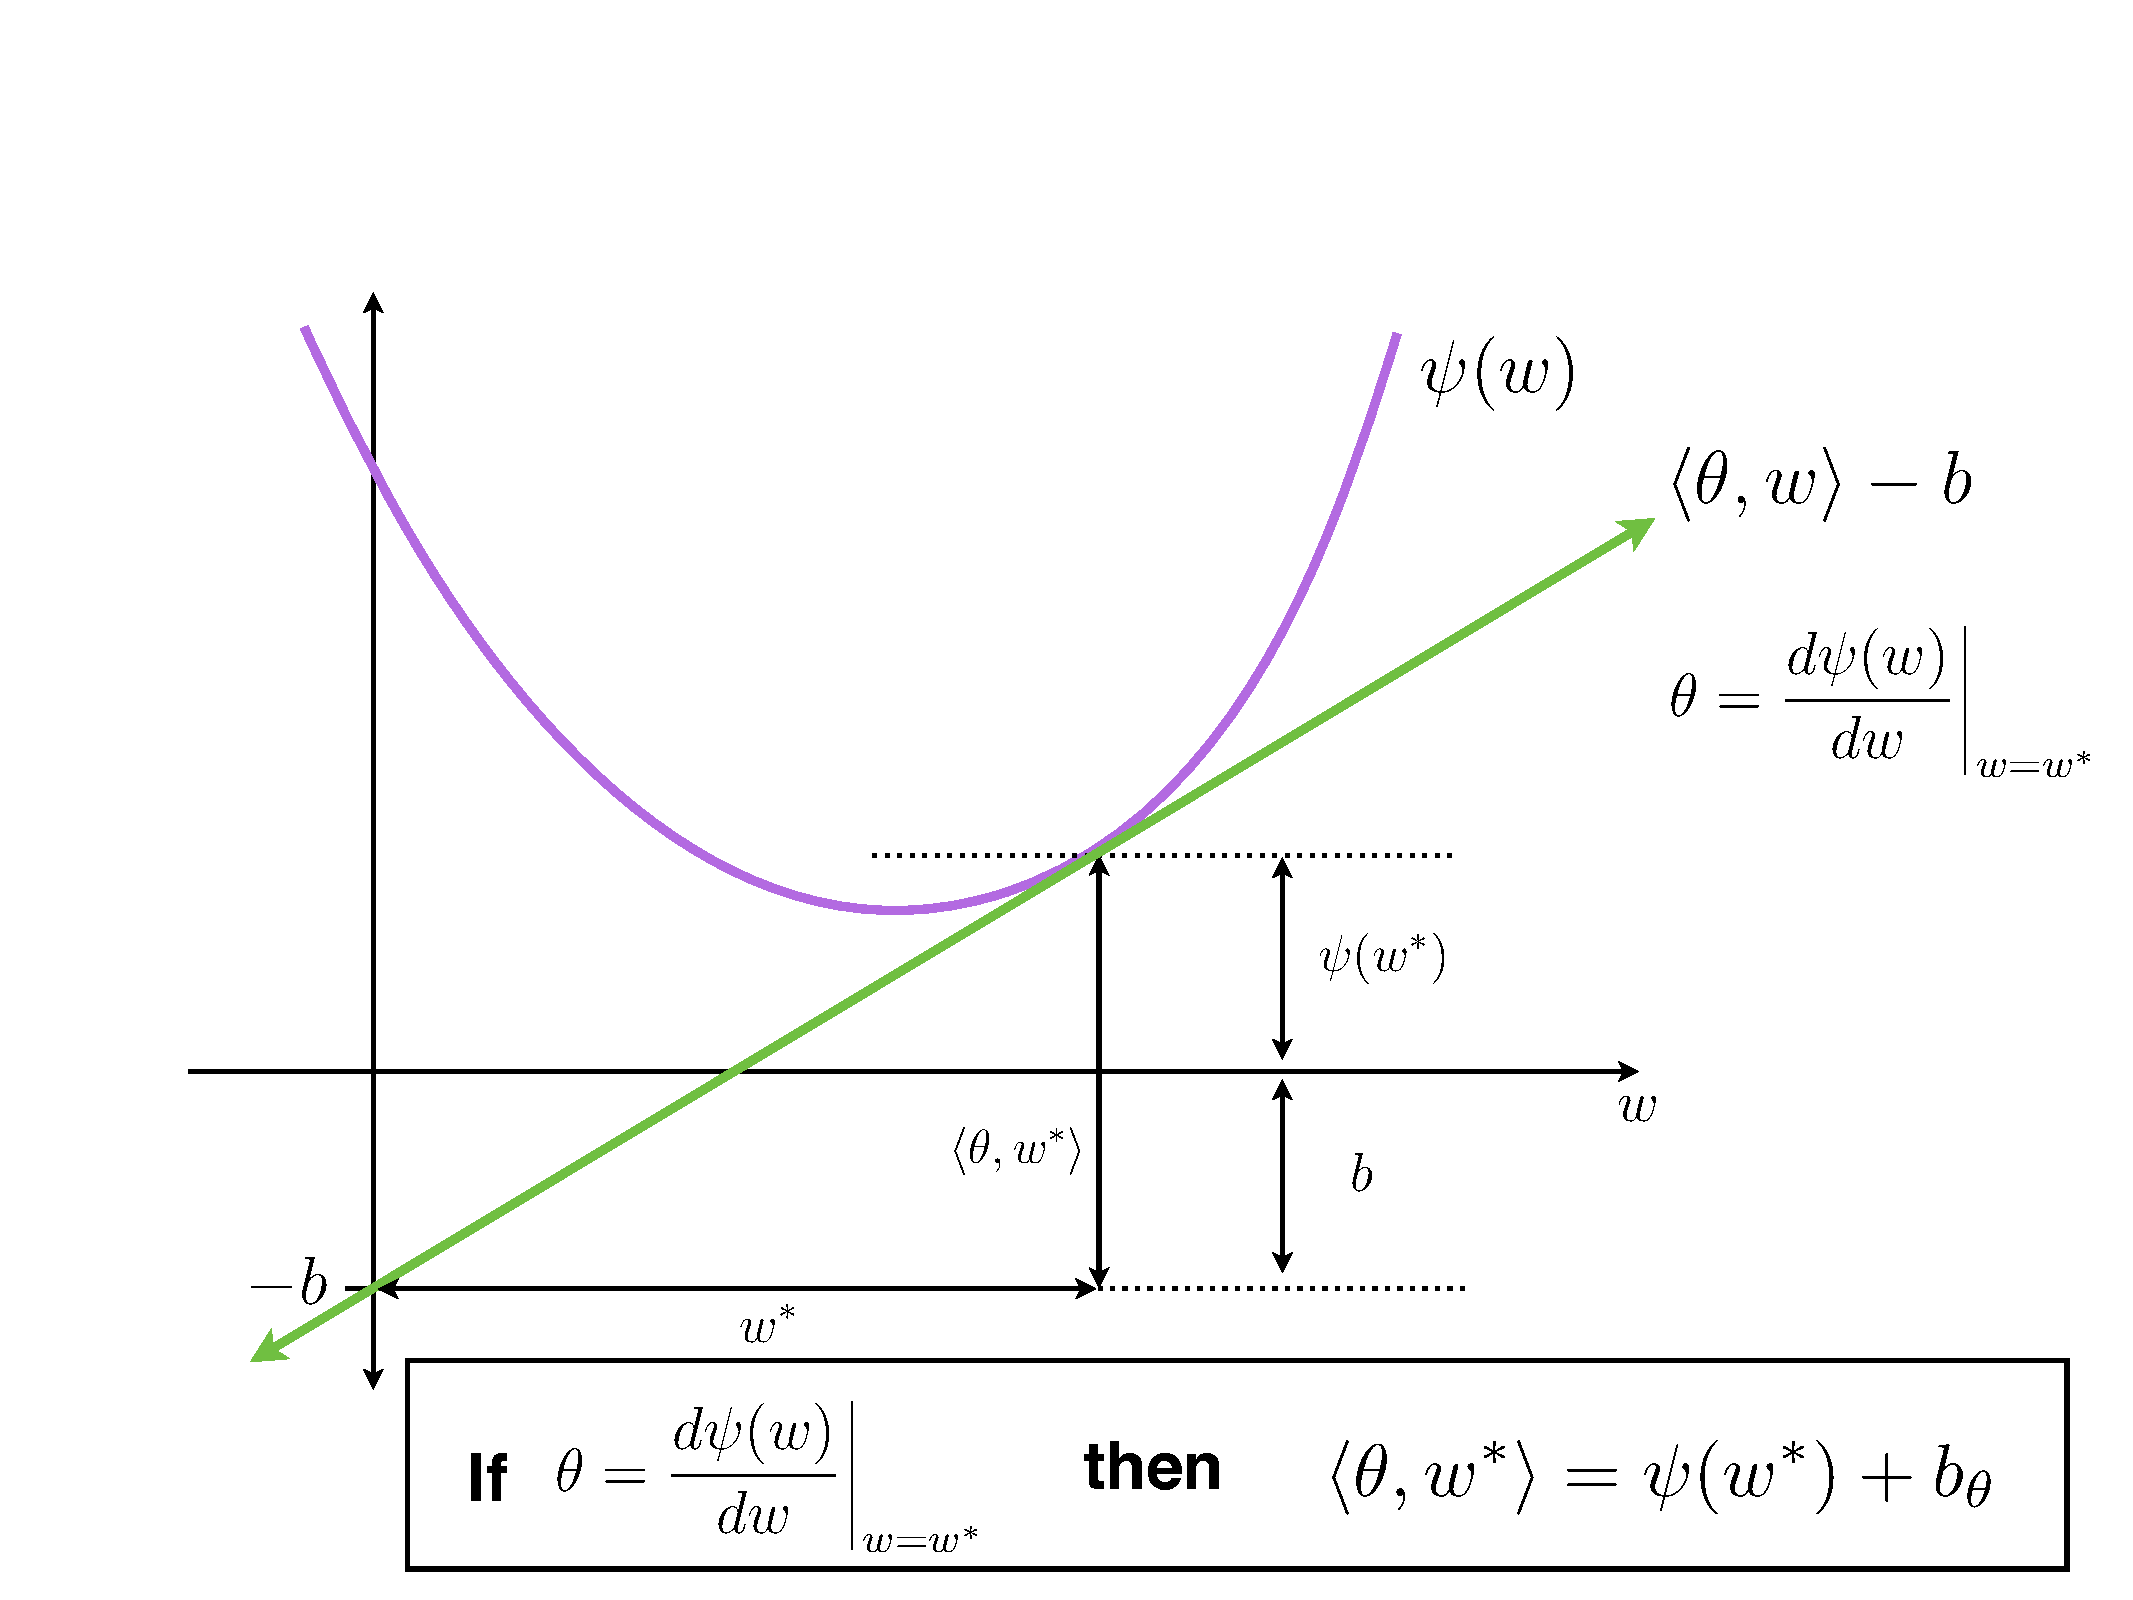
\includegraphics[width=0.65\textwidth]{figures/intercept_slope.pdf}
    \caption{Geometry of tangents}
    \label{fig:geo_tangents}
\end{figure}

As shown in Fig. \ref{fig:geo_tangents}, we have a function $\psi(w)$, and we define $\theta$ as the derivative evaluated at $w = w^*$. Then, the tangent line can be written as $\langle \theta, w \rangle - b$. So, the vertical distance (``rise'') between $-b$ and the tangent point is $\langle \theta, w \rangle$. Additionally, the vertical distance can also be written as $\psi(w^*) + b$, because of the geometry shown in the figure. So, we have:
\begin{equation}
    \langle \theta, w^* \rangle = \psi(w^*) + b(\theta)
    \label{eqn:b_theta}
\end{equation}
Where $b(\theta)$ depends on the $\theta$ at the chosen $w^*$. Rearrange (\ref{eqn:b_theta}), given $\theta$, we have:
\begin{equation}
    -b(\theta) = - \langle \theta, w^*(\theta) \rangle
    + \psi(w^*(\theta))
\end{equation}
Here we have a one-to-one mapping from $\theta$ to $w^*$ because we assume $\psi$ is convex and smooth. Otherwise, we cannot write $w^*$ as a function of $\theta$.

\subsubsection{Conjugate}

Now we discuss what is a conjugate function. Consider a slope line passing through the origin: $\langle \theta, w \rangle$, and the function $\psi(w)$. As illustrated in Fig. \ref{fig:geo_conjugate}, we want to look for the maximum distance between the two functions, i.e. $w_\theta^* = \argmax{w}(\langle \theta, w \rangle - \psi(w))$. One observation we can make is that at $w_\theta^*$, the slope of the tangent line is same as $\theta$. If we draw the tangent line (dotted), the intercept of the tangent line is actually equal to the maximum distance between two functions at $w_\theta^*$.

\begin{figure}[h]
    \centering
    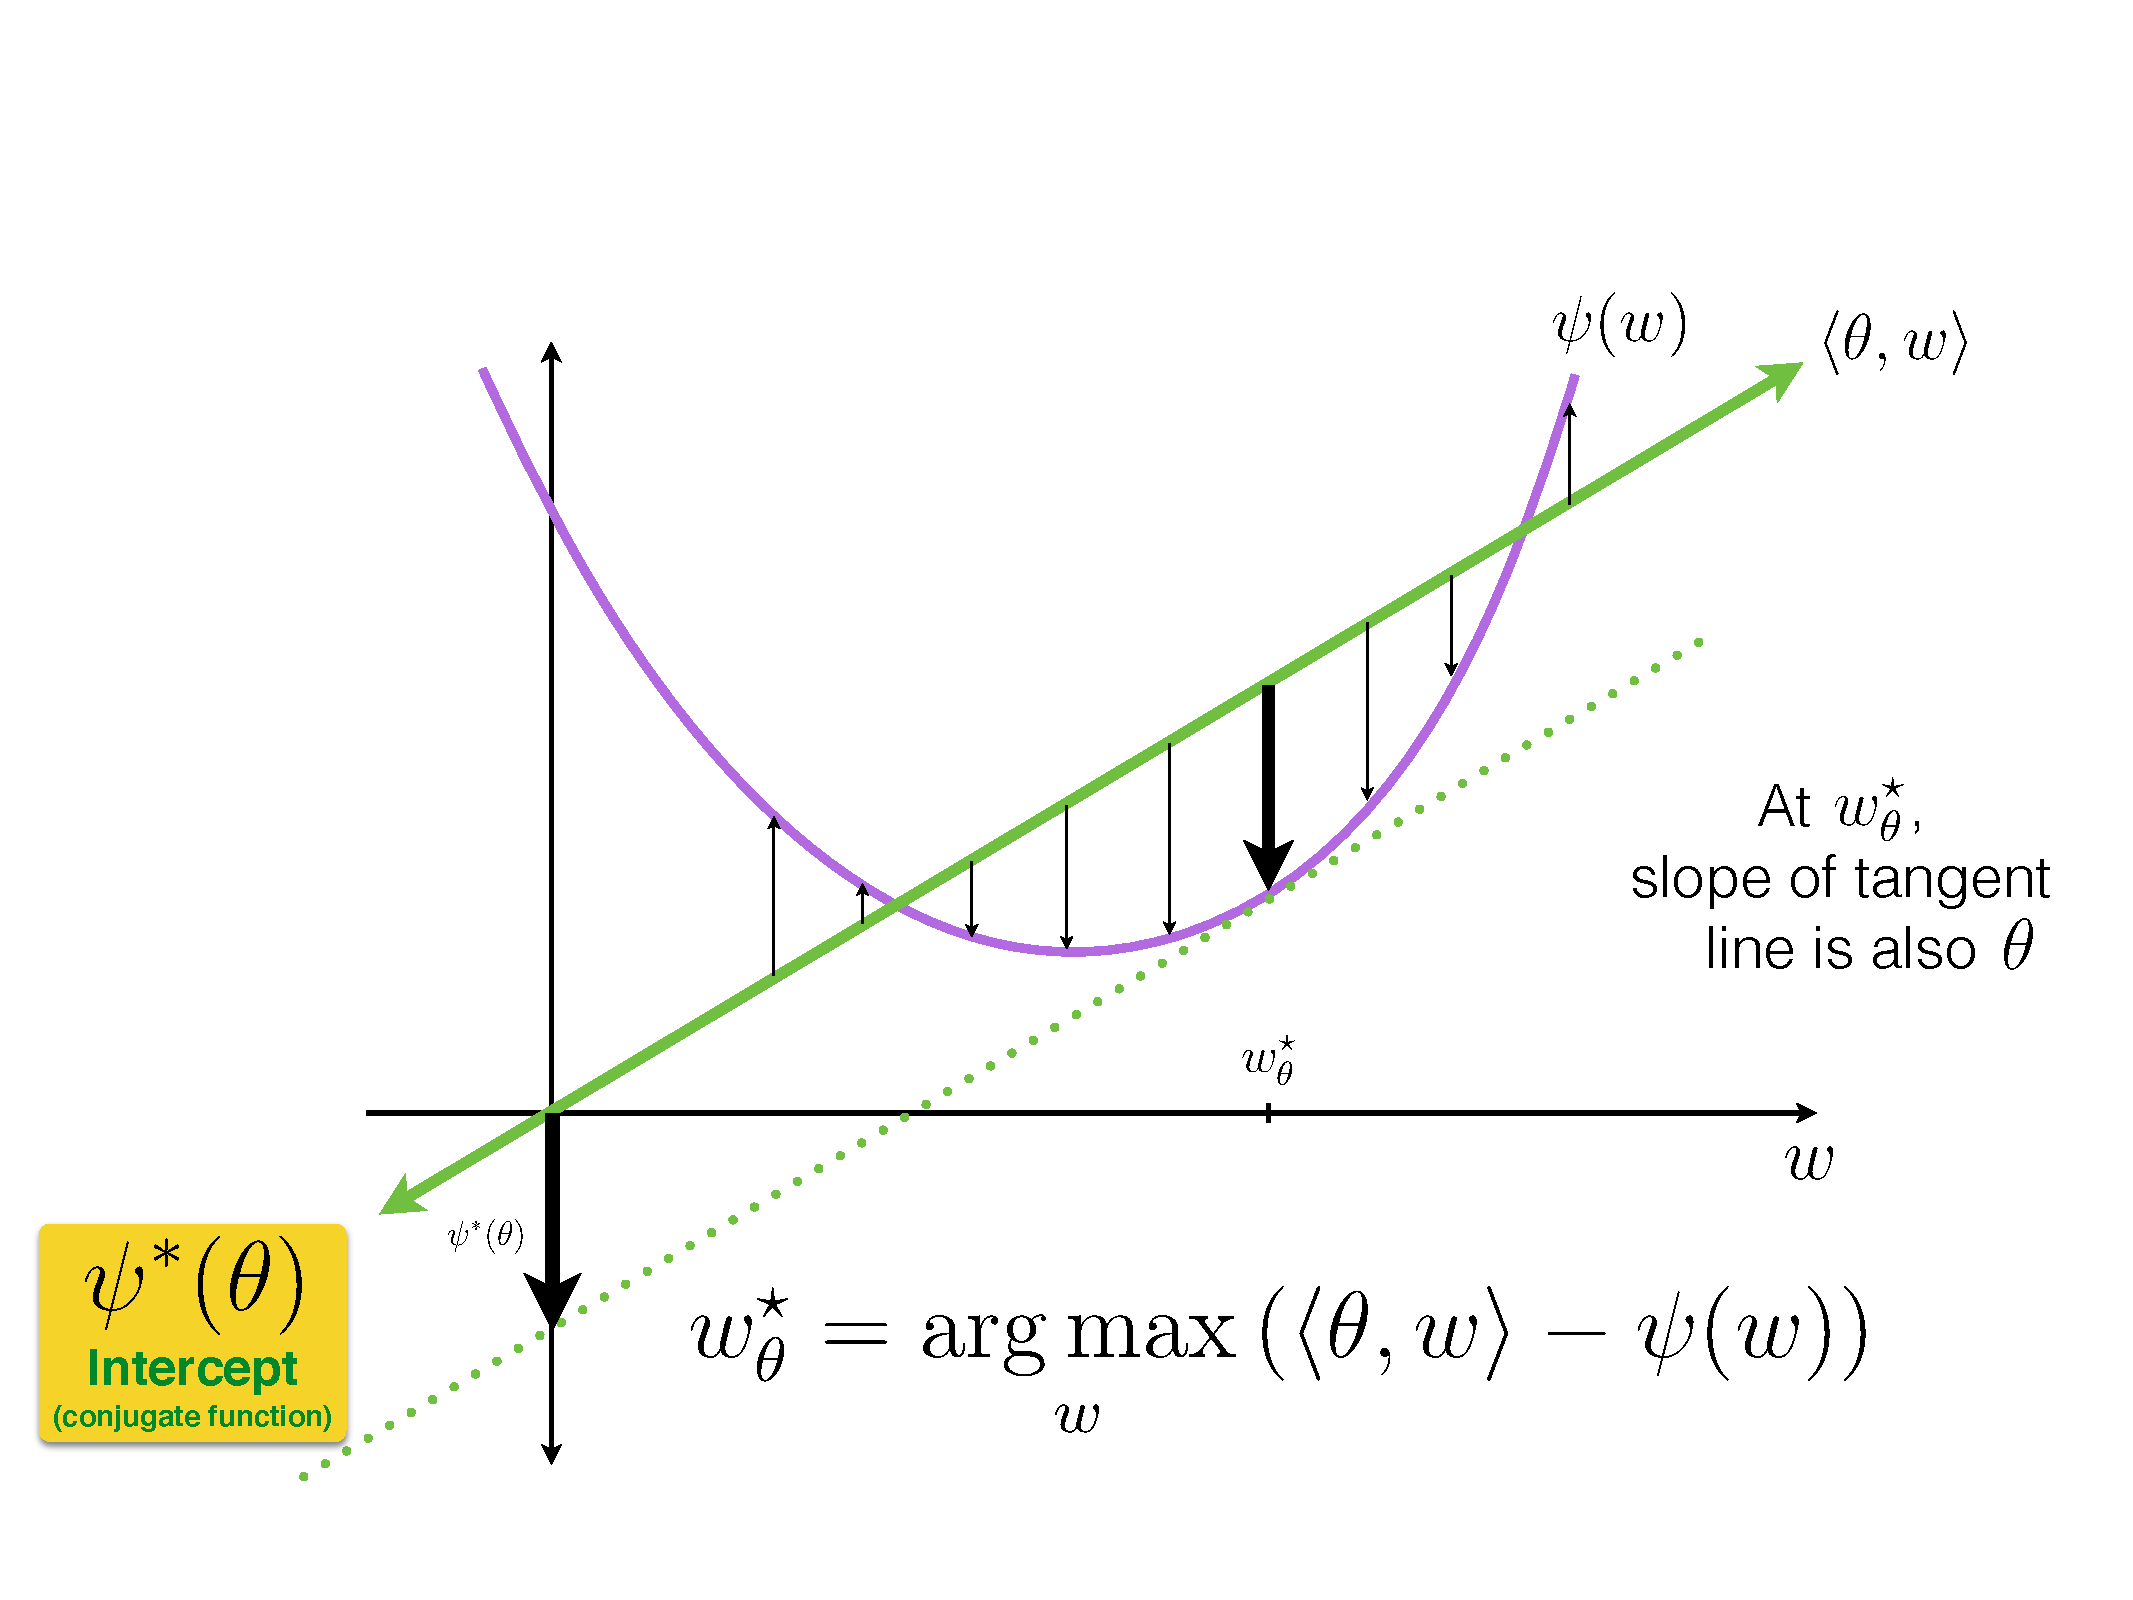
\includegraphics[width=0.75\textwidth]{figures/geom_conjugate.pdf}
    \caption{Geometry of the conjugate function $\psi^*(\theta)$}
    \label{fig:geo_conjugate}
\end{figure}

We call this maximum distance the ``intercept'' $\psi^*(\theta)$ and for any slope $\theta$, we have:
\begin{equation}
    \label{eqn:conjugate_function}
    \psi^*(\theta) = \max_w (\langle \theta, w \rangle - \psi(w))
\end{equation}
This is the geometric interpretation of the conjugate function (\ref{eqn:convex_conjugate}). To reiterate, the convex conjugate at $\theta$ is the maximum distance between function $\psi$ and the slope function $\langle \theta, w \rangle$ passing through the origin.

\subsection{Proofs for properties of convex conjugate}
\label{sec:proof_prop_conjugate}
Proof for (\ref{eqn:conjugate_deriv_2}):
\begin{proof}

\begin{align*}
    \psi^* (\bm{\theta}) &= \max_w
    (\langle \bm{\theta}, \bm{w} \rangle - \psi(\bm{w}))
    & \text{Definition (\ref{eqn:conjugate_function})}\\
    \nabla_{\bm{\theta}} \psi^* (\bm{\theta}) &=
    \nabla_{\bm{\theta}} \max_w
    (\langle \bm{\theta}, \bm{w} \rangle - \psi(\bm{w}))
    & \text{Take derivative}\\
    &= \nabla_{\bm{\theta}} (\langle \bm{\theta}, \bm{w}^* \rangle - \psi(\bm{w}^*))
    & \text{In terms of optimal $\bm{w}^*$}\\
    &= \bm{w}^*
    & \text{Compute partial derivative}
\end{align*}

\end{proof}

\subsection{Geometric interpretation of the Bregman divergence}
\label{sec:bregman_divergence_geometric}

Fig. \ref{fig:bregman_diver} shows the geometric interpretation of Bregman divergence \cite{wiki:Bregman_divergence}. $\psi(\bm{w}) - \psi(\bm{u})$ is difference of function values. $\nabla\psi(\bm{u})^\top(\bm{w}-\bm{u})$ is the first order approximation of $\psi(\bm{w})$. $D_{\psi}(\bm{w}||\bm{u})$ is the Bregman divergence.
Geometrically, it is the ``distance'' between the point on the function $\psi$ (regularization function in the case of OMD) and its tangent at $\bm{u}$ when evaluated at $\bm{w}$. It represents the first order approximation error evaluated at $\bm{w}$ with linearization point $\bm{u}$.

\begin{figure}[h]
    \centering
    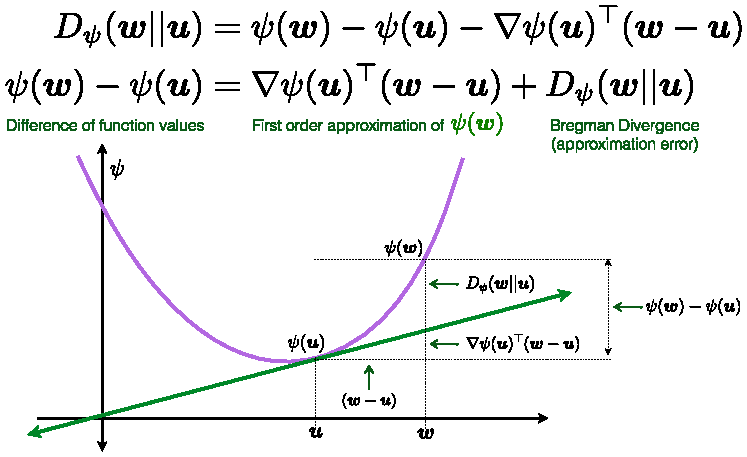
\includegraphics[width=0.8\textwidth]{figures/bregman_divergence.pdf}
    \caption{Geometric interpretation of Bregman divergence}
    \label{fig:bregman_diver}
\end{figure}



%\section{Appendix}
%This section provides any relevant background material that was not covered in the lectures, but was found to be useful for understanding the material. 
%For example, derivations, theory underlying techniques employed, etc. 

%Additionally, this section can summarizes applications or extensions of these techniques found in the literature. 

\end{document} % Done!
